\documentclass[
a4paper,                        % paper size
11pt,                           % font size
twoside,                        % two sided
footsepline,                    % add a line to separate the footer
headsepline,                    % add a line to separate the header
headexclude,                    % header does not belong to the text
footexclude,                    % footer does not belong to the text
pagesize,                       % set the pagesize in a DVI document
bibtotocnumbered,               % add the bibliography to the TOC
idxtotoc                        % add the index to the TOC
%openright,                      % start a new chapter on the right page
%,DIV12
%,draft
]{scrreprt}

\usepackage{nameref}            % nameref, varioref, hyperref must be
                                % used in this order (see hyperref
                                % README)!
\usepackage[draft]{varioref}    % defines \vref
\usepackage{hyperref}           % automatically creates links when
                                % using pdflatex, defines \url
\usepackage{ifpdf}              % defines \ifpdf
\usepackage{graphicx}           % handles graphics
\usepackage{makeidx}            % creates the index
\usepackage{fancybox}

%%%%%%%%%%%%%%%%%%%%%%%%%%%%%%%%%%%%%%%%%%%%%%%%%%
%%%%%%%%%%%%%%%%%%%%%%%%%%%%%%%%%%%%%%%%%%%%%%%%%%
%%%%%%%%% New Commands and Environments %%%%%%%%%%
%%%%%%%%%%%%%%%%%%%%%%%%%%%%%%%%%%%%%%%%%%%%%%%%%%
%%%%%%%%%%%%%%%%%%%%%%%%%%%%%%%%%%%%%%%%%%%%%%%%%%
\newcommand{\es}{\textsf{ESPResSo}}
\newcommand{\ie}{\textit{i.e.\/}}
\newcommand{\eg}{\textit{e.g.\/}}
\newcommand{\etal}{\textit{et al.\/}}

\newcommand{\variant}[2]{(#1) \texttt{#2}\\}
%\newcommand{\lit}[1]{\texttt{#1}}
\newcommand{\var}[1]{\textrm{\textit{#1}}}
\newenvironment{syntax}{%
  \begin{Sbox}
    \begin{minipage}{0.9\linewidth}
    }{%
    \end{minipage}
  \end{Sbox}
  \begin{center}
    \fbox{\TheSbox}
  \end{center}
}

%%%%%%%%%%%%%%%%%%%%%%%%%%%%%%%%%%%%%%%%%%%%%%%%%%
%%%%%%%%%%%%%%%%%%%%%%%%%%%%%%%%%%%%%%%%%%%%%%%%%%
%%%%%%%%%%%%%%%% Other Settings %%%%%%%%%%%%%%%%%%
%%%%%%%%%%%%%%%%%%%%%%%%%%%%%%%%%%%%%%%%%%%%%%%%%%
%%%%%%%%%%%%%%%%%%%%%%%%%%%%%%%%%%%%%%%%%%%%%%%%%%
\pagestyle{headings}
\makeindex

%%%%%%%%%%%%%%%%%%%%%%%%%%%%%%%%%%%%%%%%%%%%%%%%%%
%%%%%%%%%%%%%%%%%%%%%%%%%%%%%%%%%%%%%%%%%%%%%%%%%%
%%%%%%%%%%%%%%%%% Main Document %%%%%%%%%%%%%%%%%%
%%%%%%%%%%%%%%%%%%%%%%%%%%%%%%%%%%%%%%%%%%%%%%%%%%
%%%%%%%%%%%%%%%%%%%%%%%%%%%%%%%%%%%%%%%%%%%%%%%%%%
\begin{document}
\titlehead{
  \begin{center}
    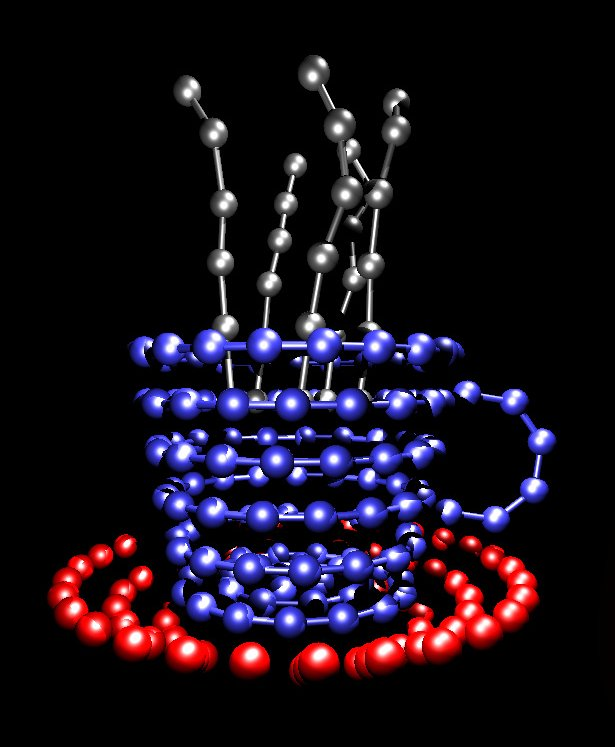
\includegraphics[width=5cm]{logo.jpg}
  \end{center}
}
%\subject{Dissertation}
\title{\es{} User's Guide}
%\author{Dipl.-Inform. Olaf~Lenz}
%\date{\today}
\maketitle

\tableofcontents

\chapter{Introduction}
\label{chap:intro}

(new)

\begin{itemize}
\item \es{} is a generic soft matter simulation packages
\item for molecular dynamics simulations in soft matter research
\item focussed on coarse-grained models
\item employs modern algorithms (Lattice-Boltzmann, DPD, P3M, \ldots)
\item written in C for maximal portability
\item Tcl-controlled
\item parallelized
\end{itemize}

\section{Guiding principles}
\label{sec:ideas}

(from paper: 2.1 Goals and principles)

\es
\begin{itemize}
\item does \emph{not} do the physics for you!
\item requires you to understand what you do (can not be used as a
  black box)
\item gives you maximal freedom (flexibility)
\item is extensible
\item integrates system setup, simulation and analysis, as this can't
  be strictly separated in soft matter simulations
\item has no predefined units
\item sets as few defaults as possible
\end{itemize}

\section{Algorithms contained in \es}

The following algorithms are implemented in \es{}:

\begin{itemize}
\item ensembles: NVE, NVT, NpT
\item charged systems:
  \begin{itemize}
  \item P3M for fully periodic systems
  \item ELC and MMM-family of algorithms for charged systems with
    non-periodic boundary conditions
  \item Maggs algorithm 
  \end{itemize}
\item Hydrodynamics:
  \begin{itemize}
  \item DPD (as a thermostat)
  \item Lattice-Boltzmann
  \end{itemize}
\end{itemize}

\section{Basic program structure}
\label{sec:structure}

(from paper: 2.2 Basic program structure)

\begin{itemize}
\item Control level: \texttt{Tcl}
\item ``Kernel'' written in \texttt{C}
\item This manual will focus on the control level
\end{itemize}

\section{On units}
\label{sec:units}

(new)

\begin{itemize}
\item Reduced units
\item comparison to ``real units''
\item three examples on different length scales
  \begin{itemize}
  \item some atomistic model?
  \item coarse-grained model (\eg lipid bilayer)
  \item billards?
  \end{itemize}
\end{itemize}

\chapter{Installation}
\label{chap:install}
\index{Installation|textbf}

\begin{itemize}
\item Compiling \es{} is a necessary evil
\item Features can be compiled in or not
\item For maximal efficiency, compile in only the features that you
  use
\item \es{} can be obtained from the \es{} home page
  \footnote{\url{http://www.espresso.mpg.de}}.
\end{itemize}



\section{Requirements}
\label{sec:requirements}
\index{requirements}

\begin{description}
\item[Tcl/Tk] \index{Tcl/Tk} \es{} requires the Toolkit Command
  Language Tcl/Tk \footnote{\url{http://www.tcl.tk/}} in the version
  8.3 or later.  Some example scripts will only work with Tcl 8.4. You
  do not only need the interpreter, but also the header files and
  libraries.  Depending on the operating system, these may come in
  separate development packages. If you want to use a graphical user
  interface (GUI) for your simulation scripts, you will also need Tk.
  
\item[FFTW] \index{FFTW} In addition, \es{} needs the FFTW library
  \footnote{\url{http://www.fftw.org/}} for Fourier transforms.
  ESPResSo can work with both the 2.1.x and 3.0.x series. Again, the
  header files are required.
  
\item[MPI] \index{MPI} Finally, if you want to use ESPResSo in
  parallel, you need a working MPI environment (version 1.2). ESPResSo
  currently supports the following MPI implementations:
  \begin{itemize}
  \item LAM/MPI is the preferred variant
  \item MPICH, which seems to be considerably slower than LAM/MPI in
    our benchmarks.
  \item On AIX systems, \es{} can also use the native POE parallel
    environment.
  \item On DEC/Compaq/HP OSF/Tru64, \es{} can also use the native
    dmpirun MPI environment.
  \end{itemize}
\end{description}

\section{Quick start}

\index{configure}\index{make}

In many cases, to compile \es{}, it is enough to execute the following
sequence of two steps in the directory where you have unpacked the
sources:
\begin{verbatim}
> configure
> make
\end{verbatim}

In some cases, \eg{} when \es{} needs to be compiled for several
different platforms or when different versions with different sets of
features are required, it might be useful to execute the commands not
in the source directory itself, but to start \texttt{configure} from
another directory (see section \vref{sec:builddir}). Furthermore, many
features of \es{} can be selectively turned on or off in the local
configuration header of \es{} (see section \vref{sec:myconfig}) before
starting the compilation with \texttt{make}.

The shell script \texttt{configure} prepares the source code for
compilation. It will determine how to use and where to find the
different libraries and tools required by the compilation process, and
it will test what compiler flags are to be used.  The script will find
out most of these things automatically.  If something is missing, it
will complain and give hints how to solve the problem.  The
configuration process can be controlled with the help of a number of
options that are explained in section \vref{sec:configure}.

The command \texttt{make} will compile the source code. Depending on
the options passed to the program, \texttt{make} can also be used for
a number of other things:
\begin{itemize}
\item It can install and uninstall the program to some other
  directories. However, normally it is not necessary to actually
  \textit{install} \es{} to run it.
\item It can test the \es{} program for correctness.
\item It can build the documentation.
\end{itemize}
The details of the usage of \texttt{make} are described in section
\vref{sec:make}.

When these steps have successfully completed, \es{} can be started
with the command (see section \vref{sec:run})
\begin{verbatim}
> Espresso
\end{verbatim}

\section{Source and build directory}
\label{sec:builddir}
\index{build directory} \index{source directory}

If you plan to use \es{} with a single configuration, you can skip the
rest of this section. If then you have problems finding the \es{}
binary or you come upon a reference to the \emph{build directory} in
the documentation, you might have to read it, anyway. In this case,
you might also want to focus on section
\vref{sec:compiling_in_srcdir}.

Usually, when a program is compiled, the resulting binary files are
put into the same directory as the sources of the program. In \es{},
the \emph{source directory} that contains all the source files can be
completely separated from the \emph{build directory} where the files
created by the build process are put. As the source directory is not
touched during the compilation process, it is possible to compile more
than one binary version of \es{} from the same set of source files.
This is useful in cases when \es{} is to be used on different computer
hardware or with a different configuration.

The source directory is the directory that contains the source files.
The location of the build directory is determined when the
\texttt{configure}-script is called.  Usually, the build directory is
assigned to the current working directory when the
\texttt{configure}-script was called. All further commands concerning
compiling and running \es{} have to be called from this directory.

\paragraph{Example}
When the source directory is \texttt{\$srcdir} (\ie{} the files where
unpacked to this directory), then the build directory can be set to
\texttt{\$builddir} by calling the \texttt{configure}-script from
there:
\begin{verbatim}
> cd $builddir
> $srcdir/configure
> make
> Espresso
\end{verbatim}

\subsection{Compiling in the source directory}
\label{sec:compiling_in_srcdir}

It is possible to run the commands \texttt{configure}, \texttt{make}
and \texttt{Espresso} directly in the source directory. In this case,
the \es{} build system is also prepared to handle different platforms.

When \texttt{configure} is from the source directory, a new
subdirectory is created and \texttt{configure} is recursively called
from this directory, making the subdirectory the build directory.  The
directory is called \texttt{obj-}\textit{platform}\texttt{/}, where
\textit{platform} is a descriptor of the CPU type where the script was
started, \eg{} \texttt{obj-Athlon\_64-pc-linux}.

Furthermore, the option \texttt{--enable-chooser} will be set in the
recursive call of \texttt{configure}, that influences how the
installed \es{} binary is found.

\section{The configuration header \texttt{myconfig.h}}
\label{sec:myconfig}

\index{myconfig.h} \index{configuration header} \es{} has a great
number of features that can be compiled into the binary (see chapter
\vref{chap:features}).  However, it is not recommended to actually
compile in all possible features, as this will negatively affect \es's
performance. Instead, compile in only the features that are actually
required. For the developers, it is also possible to turn on or off a
number of debugging messages. The features and debug messages can be
controlled via a configuration header file that contains
C-preprocessor declarations.

By default, the configuration header is called \texttt{myconfig.h}.
The name of the configuration header can be either changed when the
\texttt{configure}-script is called with the option
\texttt{--with-myconfig} (see section \vref{sec:configure}), or when
\texttt{make} is called with the setting
\texttt{myconfig=}\textit{myconfig\_header} (see section
\vref{sec:make}).

The configuration header can be put in the build directory, or in the
source directory. When a configuration header is found in both
directories, the one in the build directory will be used. If both
directories do not contain a configuration header, a default header
will be used that turns on the default features.

The file \texttt{myconfig-sample.h} in the source directory contains
an example configuration header.

\paragraph{Example}
The configuration header can be used to compile different versions
from the same source directory. Suppose that you have a source
directory \texttt{\$srcdir} and two build directories
\texttt{\$builddir1} and \texttt{\$builddir2} that contain different
configuration headers:

\begin{itemize}
\item \texttt{\$builddir1/myconfig.h}:
\begin{verbatim}
#define ELECTROSTATICS
#define LENNARD-JONES
\end{verbatim}

\item \texttt{\$builddir2/myconfig.h}:
\begin{verbatim}
#define LJCOS
\end{verbatim}
\end{itemize}

\noindent Then you can simply compile two different versions of \es{} via
\begin{verbatim}
cd $builddir1
$srcdir/configure
make

cd $builddir2
$srcdir/configure
make
\end{verbatim}

\section{Running configure}
\label{sec:configure}

\texttt{configure} will save the assembled information in the
different \texttt{Makefile}s, the header file \texttt{acconfig.h}, and
some other shell scripts required later on.

The following options are recognised by \texttt{configure}:
\begin{verbatim}
--prefix=PREFIX (Default: $HOME/Espresso)
--exec-prefix=EXEC_PREFIX (DEFAULT: PREFIX)

--enable-chooser (Default: depends on current directory)
--with-myconfig=MYCONFIG_HEADER (Default: myconfig.h)
--enable-config=KNOWN_CONFIG (Default: no)
--enable-debug (Default: off)
--enable-profiling (Default: off)
--disable-processor-optimization (Default: enabled)
--enable-xlc-qipa (Default: yes)

--with-mpi=MPI (Default: guess)
--with-efence (Default: no)
--with-tcl=VERSION (Default: guess)
--with-tk[=VERSION] (Default: no)
--with-fftw=VERSION (Default: guess)
\end{verbatim}

The following variables have an influence on the compilation:

\begin{verbatim}
CC	gives the compiler to use. Note that MPI environments often need special
	compilers rsp. wrapper scripts.
CFLAGS	flags used in the object file compilation pass. Typically you will specify
	additional include paths here, e.g. "-I/home/me/include", but also other
	compiler flags such as "-O5" are possible. In the latter case, you will
	probably want to disable the automated CPU optimization detection via
	"--disable-processor-optimization".
LDFLAGS the same as CFLAGS for the linking pass. Note that you should NOT
	specify libraries here, since for some compilers they have to appear at
	the end of the line, only additional library paths, e.g. "-L/home/me/lib".
LIBS	Use this variable to specify additional libraries to link against, e.g.
	"-lmycoollib".
\end{verbatim}

\section{Compiling, testing and installing \es}
\label{sec:make}

\begin{verbatim}
> make [all] [myconfig=MYCONFIG_HEADER]

  Compiles Espresso. 

  Variables:
  ----------
  myconfig=MYCONFIG_HEADER
    Sets the name of the local configuration header file where you can
    turn on the different features and debug messages.
    This can be useful if you want to compile Espresso with different
    sets of features from the same sources.
    WARNING:
    If you use this when compiling Espresso, it is necessary to use
    the same setting when you recompile Espresso or to call "make
    clean" before. Otherwise, you will end up with an inconsistent
    version of Espresso.
    DO NOT USE THIS WHEN YOU WORK ON THE SOURCE CODE! 
    USE configure --with-myconfig instead!

> make check [processors=PROC] [tests=TESTS]

  Runs the Espresso testsuite.

  Variables:
  ----------
  processors=PROC (Default: "1 2 3 4 6 8")
    Sets the list of processor numbers that are to be tested,
    e.g. 'make check processors="1 2"' will run the testsuite on only
    one and two processors. 

  tests=TESTS (Default: all tests)
    Sets the tests of the testsuite that are run, e.g. 
    'make check tests="madelung.tcl"' will run only the test
    madelung.tcl.

> make clean

  Deletes the files that were created during the compilation.

> make mostlyclean

  Deletes most files that were created during the compilation. Will
  keep for example the built doxygen documentation and the Espresso
  binary.

> make dist [internal=1]

  Creates a .tar.gz-file of the Espresso sources. This will include all
  source files of Espresso as they currently are in the source
  directory, i.e. it will include local changes.
  This is useful to give your version of Espresso to other people.

  Variables:
  ----------
  internal=1
    When this is give, include the "internal" directory into the
    distribution file.

> make dist-internal

  Same as "make dist internal=1"

> make install [prefix=DIR] [exec-prefix=DIR]

  Installs Espresso.

  Variables:
  ----------
  prefix=PREFIX (Default: configure option --prefix)
    Sets the directory where to install Espresso. This
    defaults to the directory given to configure.

  exec-prefix=PREFIX (Default: configure option --exec-prefix)
    Sets the directory where to install the executable files of
    Espresso. This is only required, when the executable files are to
    be installed into some architecture-specific directory. Otherwise,
    it is identical to the prefix.

> make uninstall [prefix=DIR] [exec-prefix=DIR]

  Uninstalls Espresso. The variables are identical to the variables of
  "make install".
\end{verbatim}

\section{Running \es}
\label{sec:run}

A number of wrapper scripts are used in running \es{}:
\begin{itemize}
\item The script \texttt{Espresso} in the source and build directory
  will try to run the compiled version of \es. If it is called from
  the source directory, it assumes that \es{} was also configured in
  the source directory and will try to recursively start the script in
  the corresponding \texttt{obj-PLATFORM} build directory. If it is
  called in the build directory, it will start the \es-binary with the
  right MPI implementation.
\item The chooser script \texttt{Espresso} 
  \begin{itemize}
  \item installed when \verb!--enable-chooser! was given
  \item installed to bindir
  \item tries to run the correct version of the MPI-wrapper
    \texttt{Espresso}
  \end{itemize}
\item The MPI-wrapper \texttt{Espresso}
  \begin{itemize}
  \item installed next to \es{} binary
  \item starts the binary with the right MPI implementation
  \end{itemize}
\item The \es{} binary \texttt{Espresso-bin} can also be started
  directly, however, it requires that the environment variable
  \verb!ESPRESSO_SCRIPTS! is set to the directory where the scripts
  are installed (usually \verb!$(prefix)/lib/espresso/scripts! or
  \verb!$(prefix)/share/espresso/scripts!).
\end{itemize}

\es{} can be run via
\begin{syntax}
$>$ Espresso \var{tcl\_script} \var{N\_processors} \var{args}
\end{syntax}

Note that depending on your MPI installation, MPI jobs can only be run
in the queueing system, so that ESPResSo will not run from the command
line. In that case, you may not be able to run the testsuite, or have
to directly submit the testsuite script \verb!testsuite/test.sh! to
the queueing system.


%%% Local Variables: 
%%% mode: latex
%%% TeX-master: "ug"
%%% End: 


\chapter{Tutorial}
\label{chap:tutorial}

(from \verb!erice_tutorial! or appendix A from paper)

\begin{itemize}
\item \es: script interpreter
\item interactive use (sample session)
\item script execution
\item example script
\item Reference to \verb!tutorial.tcl! (?)
\end{itemize}

\chapter{Features of \es{}}
\label{chap:features}

\chapter{\es{} command reference}
\label{chap:ref}

(most from paper and from related pages)

\begin{itemize}
\item Will contain description of all Tcl-commands
\item Reference to appendix \vref{chap:quickref}
\item basic identifiers:
  \begin{itemize}
  \item particle type
  \item bonded interaction type
  \item molecule id
  \end{itemize}
\end{itemize}


\section{\texttt{inter}: Setting up interactions}
\label{sec:inter}
\begin{syntax}
  \variant{1}
  {inter 
    \var{part\_type\_id1} 
    \var{part\_type\_id2}
    \var{inter\_type} 
    [ \var{parameters}\ldots ]
  }
  \variant{2}
  {inter 
    \var{bond\_type\_id} \var{bond\_type} [
    \var{parameters}\ldots ]
  }
  \variant{3}
  {inter}
\end{syntax}
    % \section{Creating particles}
% \label{sec:part}
% \texttt{part}

% \section{Interactions}
% \label{sec:inter}
% \texttt{inter}

% \section{Analysis}
% \label{sec:analysis}

\chapter{Under the hood}
\label{chap:underhood}

(new)

\begin{itemize}
\item Implementation issues that are interesting for the user
\item Main loop in pseudo code (for comparison)
\item from doxygen: ``Cell systems'' 
\end{itemize}


\chapter{Getting involved}
\label{chap:devel}

\begin{itemize}
\item What to do when you want to become involved
\item How to submit a bug report
\end{itemize}


\appendix
\chapter{\es{} quick reference}
\label{chap:quickref}

\begin{itemize}
\item Short reference table of all commands
\item Complete syntax of \es{} commands
\item Features required for different commands
\end{itemize}

\chapter{The MMM family of algorithms}
\label{chap:mmm}

\chapter{Maggs algorithm}
\label{chap:maggs}

\printindex

\end{document}


%%% Local Variables: 
%%% mode: latex
%%% TeX-master: t
%%% End: 
